\documentclass[11pt]{article}
\usepackage[margin=1in]{geometry}
\usepackage{amsmath,amssymb,amsthm,bm}
\usepackage{booktabs,array,longtable}
\usepackage{graphicx}
\usepackage{xcolor}
\usepackage{hyperref}
\usepackage{enumitem}

\graphicspath{{../figures/}{figures/}}

% ---------- theorem environments ----------
\theoremstyle{plain}
\newtheorem{theorem}{Theorem}
\newtheorem{proposition}[theorem]{Proposition}
\newtheorem{lemma}[theorem]{Lemma}
\theoremstyle{definition}
\newtheorem{definition}{Definition}
\newtheorem{assumption}{Assumption}

% ---------- macros ----------
\newcommand{\R}{\mathbb{R}}
\newcommand{\E}{\mathbb{E}}
\newcommand{\Var}{\operatorname{Var}}
\newcommand{\Cov}{\operatorname{Cov}}
\newcommand{\one}{\mathbf{1}}
\newcommand{\w}{\bm{w}}
\newcommand{\bmu}{\bm{\mu}}
\newcommand{\by}[1]{\quad\text{\small\color{blue!60!black}[#1]}}   % name the rule at each step: a &= b \by{linearity}
\newcommand{\owner}[2]{\par\smallskip\noindent\textit{Owner: #1 \quad Checked by: #2}\par}
\newcommand{\todo}[1]{\textcolor{red}{\textbf{TODO:} #1}}

\title{DS5020 Final Project -- Iteration 2\\[2pt]
\large Portfolio Optimization: The Math Foundation}
\author{\todo{Member 1} \and \todo{Member 2} \and \todo{Member 3} \and \todo{Member 4}\\[4pt]
\small Project Leader (Iteration 2): \todo{name}}
\date{Fall 2026}

\begin{document}
\maketitle

% =====================================================================
\section*{Task Assignment}
\begin{tabular}{@{}llll@{}}
\toprule
ID & Task & Owner & Checker \\
\midrule
D1 / Q1 & Portfolio return and risk                 & \todo{} & \todo{} \\
D2 / Q2 & $\Sigma$ is positive semi-definite         & \todo{} & \todo{} \\
D3 / Q3 & Global minimum-variance portfolio          & \todo{} & \todo{} \\
D4 / Q4 & Target-return constraint, $2\times2$ system & \todo{} & \todo{} \\
D5 / Q5 & Efficient frontier is a parabola           & \todo{} & \todo{} \\
S1      & Data loading and description               & \todo{} & \todo{} \\
S2      & Simulation check                           & \todo{} & \todo{} \\
\bottomrule
\end{tabular}

% =====================================================================
\section{Notation}
\begin{longtable}{@{}l p{8.2cm} l@{}}
\toprule
Symbol & Meaning & Dimension \\
\midrule
$N$ & number of assets (stocks) & scalar, $N=9$ \\
$T$ & number of trading days & scalar, $T=1538$ \\
$p_{t,i}$ & adjusted closing price of stock $i$ on day $t$ & scalar \\
$R_{t,i}$ & simple daily return of stock $i$ on day $t$ & scalar \\
$R$ & data matrix of returns; row $t$ = trading day, column $i$ = stock & $\R^{T\times N}$ \\
$\bm{r}_t$ & return vector on day $t$ (row $t$ of $R$, as a column) & $\R^{N}$ \\
$\bmu$ & expected return vector, $\mu_i = \E[R_i]$ & $\R^{N}$ \\
$\Sigma$ & covariance matrix, $\Sigma_{ij} = \Cov(R_i,R_j)$ & $\R^{N\times N}$ \\
$\hat\bmu,\ \hat\Sigma$ & sample mean and sample covariance & $\R^{N}$, $\R^{N\times N}$ \\
$\w$ & portfolio weights, $w_i$ = fraction of wealth in asset $i$ & $\R^{N}$ \\
$\one$ & vector of ones & $\R^{N}$ \\
$\w^*$ & global minimum-variance weights & $\R^{N}$ \\
$r$ & target expected return & scalar \\
$\lambda,\ \lambda_1,\ \lambda_2$ & Lagrange multipliers & scalars \\
$a,b,c$ & $a=\one^\top\Sigma^{-1}\one,\ b=\bmu^\top\Sigma^{-1}\one,\ c=\bmu^\top\Sigma^{-1}\bmu$ & scalars \\
$d$ & $ac-b^2$ & scalar \\
$\sigma^2_p$ & portfolio variance $\w^\top\Sigma\w$ & scalar \\
\bottomrule
\end{longtable}

\subsection*{Connecting the data to the math}
\begin{itemize}[nosep]
  \item \textbf{One row} of $R$ is one trading day $t$ between 2020-10-01 and 2026-11-13.
  \item \textbf{One column} of $R$ is one stock $i\in\{$AAPL, NVDA, GOOGL, META, AMZN, AMD, PLTR, MU, INTC$\}$.
  \item \textbf{One entry} $R_{t,i} = (p_{t,i}-p_{t-1,i})/p_{t-1,i}$ is the return of stock $i$ on day $t$, computed from adjusted closing prices (so splits and dividends are accounted for).
  \item \textbf{One weight} $w_i$ is the fraction of wealth held in stock $i$; $w_i<0$ means a short position.
\end{itemize}

% =====================================================================
\section{Definitions}
\begin{definition}[Random vector, expectation]\todo{}\end{definition}
\begin{definition}[Covariance and covariance matrix]\todo{$\Sigma = \E[(\bm r-\bmu)(\bm r-\bmu)^\top]$}\end{definition}
\begin{definition}[Sample mean and sample covariance]\todo{$\hat\Sigma = \frac{1}{T-1}R_c^\top R_c$, $R_c = R - \one\hat\bmu^\top$}\end{definition}
\begin{definition}[Symmetric, positive (semi-)definite matrix]\todo{}\end{definition}
\begin{definition}[Portfolio, budget constraint $\one^\top\w = 1$]\todo{}\end{definition}
\begin{definition}[Gradient of $\w^\top A\w$ and $\bm{c}^\top\w$]\todo{}\end{definition}
\begin{definition}[Lagrangian and Lagrange multiplier]\todo{}\end{definition}
\begin{definition}[Efficient frontier]\todo{}\end{definition}

% =====================================================================
\section{Assumptions}
\begin{longtable}{@{}p{3.6cm} p{5.6cm} p{5.4cm}@{}}
\toprule
Assumption & What breaks if it fails & How we check it (Iteration 3) \\
\midrule
A1. $\bmu,\Sigma$ constant over time (stationarity) & $\hat\bmu,\hat\Sigma$ estimate an average of changing quantities; optimal weights are not optimal out of sample & \todo{rolling-window estimates of $\hat\bmu,\hat\Sigma$} \\
A2. $\Sigma$ positive definite (no redundant asset) & $\Sigma^{-1}$ does not exist; $\w^*$ and $a,b,c$ undefined & \todo{smallest eigenvalue / condition number of $\hat\Sigma$} \\
A3. $T > N$ & $\hat\Sigma$ has rank $\le T-1 < N$, so it is singular & \todo{check $T$ vs $N$} \\
A4. $\bmu$ not a multiple of $\one$ & $d = ac-b^2 = 0$; the $2\times2$ system is singular & \todo{check $d>0$} \\
A5. Investors care only about mean and variance (or returns jointly normal) & variance misses skewness / fat tails & histograms, QQ-plots, kurtosis. Already visible: excess kurtosis of daily returns is 3.8--17.9 (META 17.9, INTC 10.5), far from 0 for a normal \\
A6. Short selling allowed, no transaction costs & constrained problem has no closed form & \todo{report negative weights} \\
\bottomrule
\end{longtable}

% =====================================================================
\section{Derivations}
% Rule: name the rule used at EVERY step with \by{...}.

\begin{proposition}[Portfolio return and risk]\label{prop:q1}
For $\w\in\R^N$ and random returns $\bm r$ with mean $\bmu$ and covariance $\Sigma$,
\[
\E\Big[\textstyle\sum_i w_iR_i\Big] = \w^\top\bmu, \qquad
\Var\Big(\textstyle\sum_i w_iR_i\Big) = \w^\top\Sigma\w .
\]
\end{proposition}
\begin{proof}
\todo{Linearity of expectation; $\Var(\sum_i X_i)=\sum_i\sum_j\Cov(X_i,X_j)$; bilinearity of covariance; write the double sum as a quadratic form.}
\end{proof}
\owner{\todo{}}{\todo{}}

\begin{proposition}[$\Sigma$ is positive semi-definite]\label{prop:q2}
$\Sigma$ (and $\hat\Sigma$) is symmetric and $\bm z^\top\Sigma\bm z\ge 0$ for all $\bm z\in\R^N$. Hence portfolio risk is never negative.
\end{proposition}
\begin{proof}
\todo{Symmetry from $\Cov(X,Y)=\Cov(Y,X)$; $\bm z^\top\Sigma\bm z = \Var(\bm z^\top\bm r)\ge0$; for $\hat\Sigma$: $\bm z^\top\hat\Sigma\bm z = \frac{1}{T-1}\|R_c\bm z\|^2$.}
\end{proof}
\owner{\todo{}}{\todo{}}

\begin{theorem}[Global minimum-variance portfolio]\label{thm:q3}
If $\Sigma$ is positive definite, the solution of $\min_{\w}\ \w^\top\Sigma\w$ subject to $\one^\top\w=1$ is
\[
\w^* = \frac{\Sigma^{-1}\one}{\one^\top\Sigma^{-1}\one}, \qquad \sigma^2_{\min} = \frac{1}{\one^\top\Sigma^{-1}\one}.
\]
\end{theorem}
\begin{proof}
\todo{Lagrangian $L(\w,\lambda)=\w^\top\Sigma\w-\lambda(\one^\top\w-1)$; $\nabla_\w L = 2\Sigma\w-\lambda\one=0$; solve for $\w$; use constraint to find $\lambda$; argue it is a minimum (convexity, Prop.~\ref{prop:q2}).}
\end{proof}
\owner{\todo{}}{\todo{}}

\begin{theorem}[Target-return portfolio]\label{thm:q4}
Assume $\Sigma$ is positive definite (A2) and $\bmu$ is not a multiple of $\one$ (A4). Then for every $r\in\R$ the problem
\[
\min_{\w\in\R^N}\ \tfrac12\w^\top\Sigma\w \quad\text{subject to}\quad \bmu^\top\w=r,\quad \one^\top\w=1
\]
has the unique solution $\w = \Sigma^{-1}(\lambda_1\bmu+\lambda_2\one)$, where $(\lambda_1,\lambda_2)$ is the unique solution of the $2\times 2$ system
\[
\begin{bmatrix} c & b\\ b & a\end{bmatrix}\begin{bmatrix}\lambda_1\\ \lambda_2\end{bmatrix} = \begin{bmatrix} r\\ 1\end{bmatrix},
\qquad a=\one^\top\Sigma^{-1}\one,\ \ b=\bmu^\top\Sigma^{-1}\one,\ \ c=\bmu^\top\Sigma^{-1}\bmu .
\]
(The factor $\tfrac12$ does not change the minimizer, since multiplying an objective by a positive constant preserves the ordering of its values.)
\end{theorem}

\begin{proof}
\textbf{Step 1 (Lagrangian).} With one multiplier per equality constraint,
\[
L(\w,\lambda_1,\lambda_2) = \tfrac12\w^\top\Sigma\w - \lambda_1(\bmu^\top\w - r) - \lambda_2(\one^\top\w - 1).
\by{Def.\ of Lagrangian}
\]

\textbf{Step 2 (Stationarity).} Setting the gradient with respect to $\w$ to zero:
\begin{align*}
\nabla_{\w}L &= \tfrac12(\Sigma+\Sigma^\top)\w - \lambda_1\bmu - \lambda_2\one
  \by{$\nabla_{\w}(\w^\top A\w)=(A+A^\top)\w$,\ $\nabla_{\w}(\bm c^\top\w)=\bm c$} \\
&= \Sigma\w - \lambda_1\bmu - \lambda_2\one = \bm 0
  \by{$\Sigma=\Sigma^\top$ (Prop.~\ref{prop:q2})}
\end{align*}
so
\begin{equation}\label{eq:stationary}
\Sigma\w = \lambda_1\bmu + \lambda_2\one .
\end{equation}

\textbf{Step 3 (Solve for $\w$).} $\Sigma$ is invertible: if $\Sigma\bm x=\bm 0$ then $\bm x^\top\Sigma\bm x=0$, which forces $\bm x=\bm 0$ because $\Sigma$ is positive definite; so $N(\Sigma)=\{\bm 0\}$.\by{Def.\ of PD; invertible $\iff$ trivial null space}
Multiplying \eqref{eq:stationary} on the left by $\Sigma^{-1}$:
\begin{equation}\label{eq:w}
\w = \lambda_1\Sigma^{-1}\bmu + \lambda_2\Sigma^{-1}\one . \by{left-multiply by $\Sigma^{-1}$}
\end{equation}

\textbf{Step 4 (Impose the constraints).} First note that $\Sigma^{-1}$ is symmetric, since $(\Sigma^{-1})^\top=(\Sigma^\top)^{-1}=\Sigma^{-1}$, so
$\one^\top\Sigma^{-1}\bmu = (\one^\top\Sigma^{-1}\bmu)^\top = \bmu^\top\Sigma^{-1}\one = b$.\by{a scalar equals its transpose}
Substituting \eqref{eq:w} into the return constraint:
\begin{align*}
r = \bmu^\top\w &= \lambda_1\,\bmu^\top\Sigma^{-1}\bmu + \lambda_2\,\bmu^\top\Sigma^{-1}\one
  \by{linearity of matrix multiplication} \\
&= c\,\lambda_1 + b\,\lambda_2 . \by{def.\ of $b,c$}
\end{align*}
Substituting \eqref{eq:w} into the budget constraint:
\begin{align*}
1 = \one^\top\w &= \lambda_1\,\one^\top\Sigma^{-1}\bmu + \lambda_2\,\one^\top\Sigma^{-1}\one
  \by{linearity} \\
&= b\,\lambda_1 + a\,\lambda_2 . \by{symmetry of $\Sigma^{-1}$; def.\ of $a,b$}
\end{align*}
Together these are exactly the $2\times2$ system in the theorem.

\textbf{Step 5 (The $2\times2$ system has a unique solution).} Its determinant is $d=ac-b^2$. Because $\Sigma^{-1}$ is positive definite (its eigenvalues are $1/\lambda_i>0$), $\langle\bm x,\bm y\rangle := \bm x^\top\Sigma^{-1}\bm y$ is an inner product on $\R^N$.\by{symmetric, bilinear, $\langle\bm x,\bm x\rangle>0$ for $\bm x\neq\bm 0$}
Then $a=\langle\one,\one\rangle$, $b=\langle\bmu,\one\rangle$, $c=\langle\bmu,\bmu\rangle$, and
\[
b^2 = \langle\bmu,\one\rangle^2 \le \langle\bmu,\bmu\rangle\langle\one,\one\rangle = ca,
\by{Cauchy--Schwarz}
\]
with equality only if $\bmu$ and $\one$ are linearly dependent. By A4 they are not, so $d=ac-b^2>0$, the matrix is invertible, and $(\lambda_1,\lambda_2)$ exists and is unique.\by{$\det\neq0\iff$ invertible}

\textbf{Step 6 (It is the minimum, and it is unique).} Let $\w$ be the point from Steps 3--5 and let $\w'=\w+\bm h$ be any other feasible point. Both satisfy the constraints, so $\bmu^\top\bm h=0$ and $\one^\top\bm h=0$.\by{subtract the constraints}
Then
\begin{align*}
\tfrac12\w'^\top\Sigma\w' &= \tfrac12\w^\top\Sigma\w + \bm h^\top\Sigma\w + \tfrac12\bm h^\top\Sigma\bm h
  \by{expand; $\bm h^\top\Sigma\w=\w^\top\Sigma\bm h$ by symmetry} \\
&= \tfrac12\w^\top\Sigma\w + \bm h^\top(\lambda_1\bmu+\lambda_2\one) + \tfrac12\bm h^\top\Sigma\bm h
  \by{eq.~\eqref{eq:stationary}} \\
&= \tfrac12\w^\top\Sigma\w + \tfrac12\bm h^\top\Sigma\bm h
  \by{$\bmu^\top\bm h=\one^\top\bm h=0$} \\
&> \tfrac12\w^\top\Sigma\w \quad\text{whenever } \bm h\neq\bm 0 .
  \by{$\Sigma$ positive definite}
\end{align*}
So every other feasible portfolio has strictly larger variance: $\w$ is the unique minimizer.
\end{proof}
\owner{\todo{}}{\todo{}}

\begin{theorem}[The efficient frontier is a parabola]\label{thm:q5}
Under the assumptions of Theorem~\ref{thm:q4}, with $d=ac-b^2>0$, the minimum variance at target return $r$ is
\[
\sigma^2(r) = \frac{a r^2 - 2 b r + c}{d}
= \frac{a}{d}\Big(r-\frac{b}{a}\Big)^2 + \frac{1}{a},
\]
a parabola in the $(\sigma^2, r)$ plane that opens toward larger $\sigma^2$, with vertex at $\big(\sigma^2,r\big)=\big(1/a,\ b/a\big)$. The vertex is the global minimum-variance portfolio $\w^*$ of Theorem~\ref{thm:q3}.
\end{theorem}

\begin{proof}
Let $\w$ be the minimizer from Theorem~\ref{thm:q4} for target $r$.

\textbf{Step 1 (Variance in terms of the multipliers).}
\begin{align*}
\sigma^2(r) = \w^\top\Sigma\w &= \w^\top(\lambda_1\bmu + \lambda_2\one)
  \by{eq.~\eqref{eq:stationary}} \\
&= \lambda_1\,\w^\top\bmu + \lambda_2\,\w^\top\one
  \by{linearity} \\
&= \lambda_1 r + \lambda_2 .
  \by{constraints $\bmu^\top\w=r$, $\one^\top\w=1$}
\end{align*}

\textbf{Step 2 (Solve the $2\times2$ system).} Since $d\neq0$ (Theorem~\ref{thm:q4}, Step 5),
\[
\lambda_1 = \frac{\det\begin{bmatrix} r & b\\ 1 & a\end{bmatrix}}{d} = \frac{ar-b}{d},
\qquad
\lambda_2 = \frac{\det\begin{bmatrix} c & r\\ b & 1\end{bmatrix}}{d} = \frac{c-br}{d}.
\by{Cramer's rule}
\]

\textbf{Step 3 (Substitute).}
\begin{align*}
\sigma^2(r) &= r\cdot\frac{ar-b}{d} + \frac{c-br}{d}
  \by{Steps 1 and 2} \\
&= \frac{ar^2 - 2br + c}{d}.
  \by{common denominator, collect terms}
\end{align*}

\textbf{Step 4 (Complete the square).}
\begin{align*}
ar^2 - 2br + c &= a\Big(r^2 - \frac{2b}{a}r\Big) + c
  \by{factor out $a$; $a=\langle\one,\one\rangle>0$} \\
&= a\Big(r-\frac{b}{a}\Big)^2 - \frac{b^2}{a} + c
  \by{completing the square} \\
&= a\Big(r-\frac{b}{a}\Big)^2 + \frac{d}{a},
  \by{$c-\tfrac{b^2}{a}=\tfrac{ac-b^2}{a}$}
\end{align*}
so, dividing by $d$,
\[
\sigma^2(r) = \frac{a}{d}\Big(r-\frac{b}{a}\Big)^2 + \frac{1}{a}.
\]
This has the form $\sigma^2 = \alpha(r-r_0)^2+\beta$ with $\alpha=a/d>0$, which is a parabola in the $(\sigma^2,r)$ plane: its axis is horizontal (the line $r=r_0=b/a$), it opens toward larger $\sigma^2$, and its vertex is at $(\beta,r_0)=(1/a,\ b/a)$.\by{standard form of a parabola}
Every target $r\neq b/a$ needs strictly more variance than $1/a$, because $(r-b/a)^2>0$.

\textbf{Step 5 (The vertex is $\w^*$).} At $r=b/a$, Step 2 gives
\[
\lambda_1 = \frac{a\cdot\frac{b}{a}-b}{d}=0,\qquad
\lambda_2 = \frac{c-\frac{b^2}{a}}{d}=\frac{ac-b^2}{ad}=\frac1a,
\]
so by eq.~\eqref{eq:w}, $\w=\frac{1}{a}\Sigma^{-1}\one = \dfrac{\Sigma^{-1}\one}{\one^\top\Sigma^{-1}\one}=\w^*$, and $\sigma^2=1/a=\sigma^2_{\min}$, matching Theorem~\ref{thm:q3}.
\end{proof}

\noindent\textit{Remark.} Only the upper branch $r\ge b/a$ is \emph{efficient}: for $r<b/a$ the portfolio with return $2b/a - r$ has the same variance and a higher return. In the $(\sigma,r)$ plane, with $\sigma=\sqrt{\sigma^2}$, the same curve is a hyperbola, as in Figure~\ref{fig:frontier}.
\textit{Numerical check (simulation, $T=2000$):} $a=155.96$, $b=9.0178$, so the vertex is at $b/a=0.05782$, which equals $\w^{*\top}\hat\bmu$; the closed form matches $\w^\top\hat\Sigma\w$ to within $10^{-16}$ at every target $r$.
\owner{\todo{}}{\todo{}}

% =====================================================================
\section{Iteration 2 -- Math Questions}
\begin{enumerate}[label=\textbf{Q\arabic*.}]
  \item Derive portfolio return $\w^\top\bmu$ and risk $\w^\top\Sigma\w$ from $\Var(\sum_i w_iR_i)$. \hfill See Proposition~\ref{prop:q1}.
  \item Prove that $\Sigma$ is positive semi-definite, so risk is never negative. \hfill See Proposition~\ref{prop:q2}.
  \item Minimize $\w^\top\Sigma\w$ subject to $\one^\top\w=1$ and derive $\w^*$. \hfill See Theorem~\ref{thm:q3}.
  \item Add $\w^\top\bmu=r$; derive the $2\times2$ system for the multipliers. \hfill See Theorem~\ref{thm:q4}.
  \item Show the efficient frontier is a parabola in $(\sigma^2,r)$. \hfill See Theorem~\ref{thm:q5}.
\end{enumerate}

% =====================================================================
\section{The Algorithm as Math}
Input $R\in\R^{T\times N}$, target returns $r_1,\dots,r_K$.
\begin{enumerate}[label=(\arabic*)]
  \item $\hat\bmu = \frac1T R^\top\one_T$. \hfill sizes $N\times T$, $T$; \ $\approx NT$ flops.
  \item $R_c = R - \one_T\hat\bmu^\top$. \hfill $T\times N$; \ $NT$ flops.
  \item $\hat\Sigma = \frac{1}{T-1}R_c^\top R_c$. \hfill $N\times N$; \ $\approx 2N^2T$ flops (or $N^2T$ using symmetry).
  \item Solve $\hat\Sigma\bm x = \one$ and $\hat\Sigma\bm y = \hat\bmu$ (one LU / Cholesky factorization, two triangular solves). \hfill $\approx \frac23N^3 + 4N^2$ flops (Cholesky: $\frac13N^3$).
  \item $a=\one^\top\bm x,\ b=\hat\bmu^\top\bm x,\ c=\hat\bmu^\top\bm y,\ d=ac-b^2$. \hfill $\approx 6N$ flops.
  \item $\w^* = \bm x / a$. \hfill $N$ flops.
  \item For each $r_k$: solve $\begin{bmatrix}c&b\\b&a\end{bmatrix}\bm\lambda = \begin{bmatrix}r_k\\1\end{bmatrix}$, then $\w_k = \lambda_1\bm y + \lambda_2\bm x$ and $\sigma^2_k=\lambda_1 r_k+\lambda_2$. \hfill $O(N)$ flops each.
\end{enumerate}
Total cost: $O(N^2T + N^3 + KN)$; for $N=10$ the $N^2T$ term dominates.

% =====================================================================
\section{Data}
\textbf{Source.} Adjusted daily closing prices from Yahoo Finance (via \texttt{yfinance}) for nine large US technology stocks: AAPL, NVDA, GOOGL, META, AMZN, AMD, PLTR, MU, INTC. The window starts on 2020-09-30, PLTR's first trading day, so every stock is observed on every date. SpaceX (SPCX) was considered but dropped: it has traded only since its 2026-06-12 IPO ($\approx$107 daily returns), which would shrink the common window too much.

\textbf{Size and types.} After computing returns, $R$ has $T=1538$ rows (trading days 2020-10-01 to 2026-11-13) and $N=9$ columns, all \texttt{float64}. There are no missing values; all nine stocks trade on the same exchange calendar.

\begin{center}
\begin{tabular}{@{}lrrrr@{}}
\toprule
Stock & Ann.\ mean & Ann.\ vol. & Skew & Excess kurt. \\
\midrule
AAPL  & 0.228 & 0.279 & 0.34  & 5.7 \\
NVDA  & 0.533 & 0.501 & 0.48  & 4.5 \\
GOOGL & 0.280 & 0.314 & 0.00  & 4.0 \\
META  & 0.243 & 0.432 & $-0.08$ & 17.9 \\
AMZN  & 0.148 & 0.350 & 0.34  & 5.7 \\
AMD   & 0.463 & 0.560 & 0.46  & 4.4 \\
PLTR  & 0.707 & 0.697 & 1.13  & 6.8 \\
MU    & 0.615 & 0.551 & 0.27  & 3.8 \\
INTC  & 0.187 & 0.539 & 0.06  & 10.5 \\
\bottomrule
\end{tabular}
\end{center}
Annualized with 252 trading days: mean $\times 252$, volatility $\times\sqrt{252}$.

\textbf{First look at $\hat\Sigma$.} All eigenvalues of $\hat\Sigma$ are positive (from $1.6\times10^{-4}$ to $4.2\times10^{-3}$), consistent with Proposition~\ref{prop:q2}; its condition number is 26, so $\hat\Sigma^{-1}$ is well defined (Assumption A2). $T=1538 \gg N=9$ (Assumption A3).

\begin{figure}[h]\centering
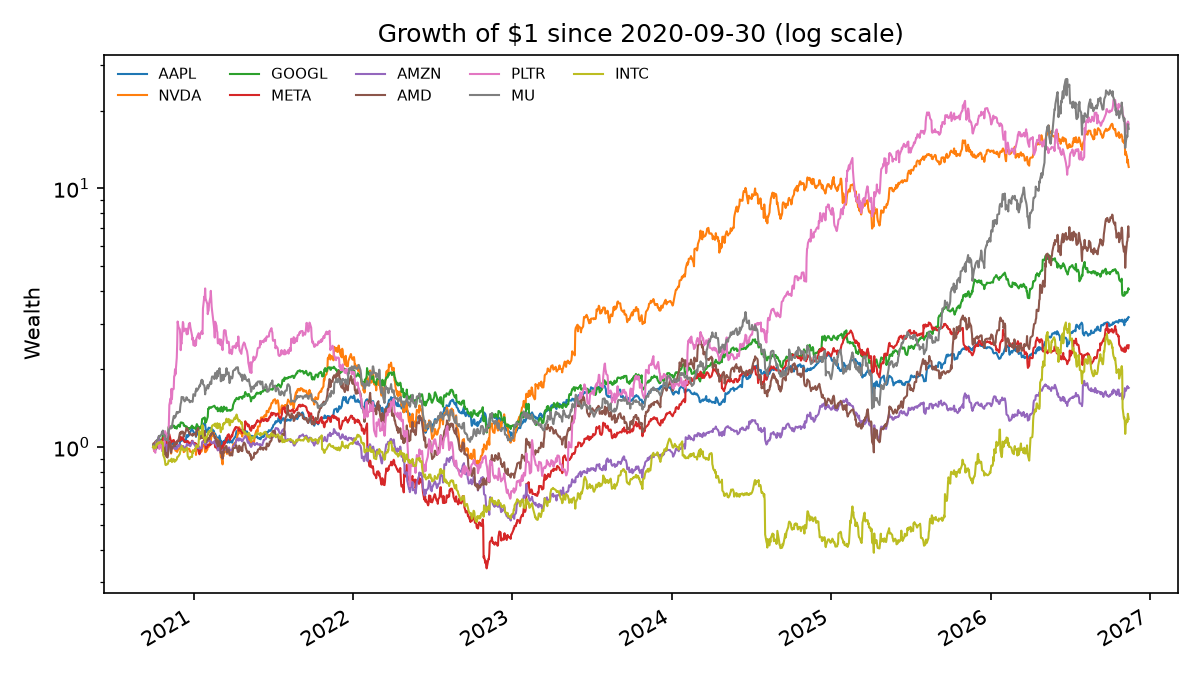
\includegraphics[width=0.85\linewidth]{data_cumulative.png}
\caption{Growth of \$1 invested in each stock on 2020-09-30 (log scale).}
\end{figure}
\begin{figure}[h]\centering
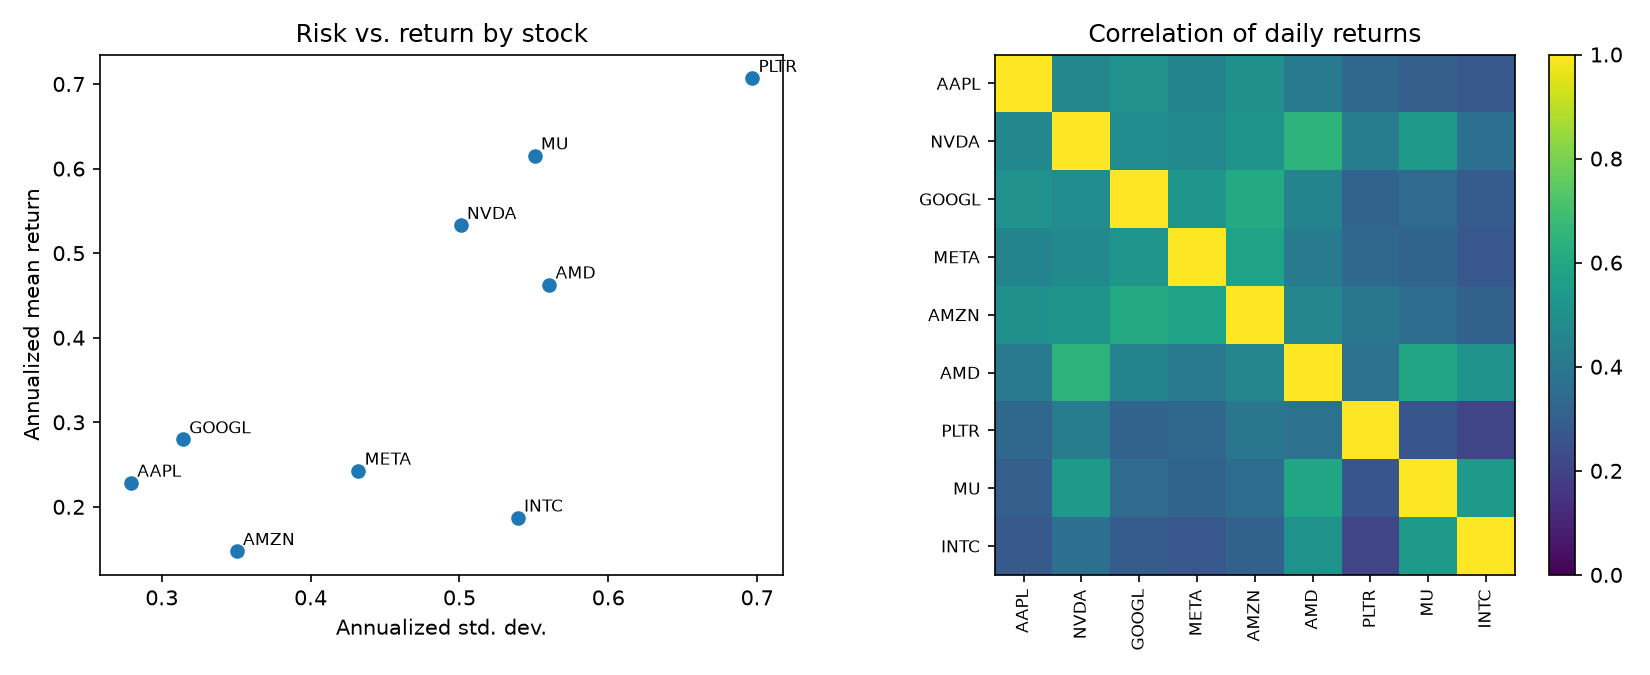
\includegraphics[width=\linewidth]{data_risk_return_corr.png}
\caption{Left: annualized mean vs.\ standard deviation. Right: correlation matrix of daily returns.}
\end{figure}

% =====================================================================
\section{Simulation}
\subsection*{Simulation Check}
\textbf{Model.} $\bm r_t \overset{\text{iid}}{\sim}\mathcal N(\bmu,\Sigma)$, $N=4$, $T=2000$, seed \texttt{default\_rng(0)}, with
$\bmu=(0.05,0.08,0.12,0.07)^\top$, volatilities $(0.10,0.15,0.25,0.12)$, and $\Sigma = \operatorname{diag}(\text{vol})\,C\,\operatorname{diag}(\text{vol})$ for the correlation matrix $C$ in \texttt{src/simulate.py}.

\begin{center}
\begin{tabular}{@{}lrrrr@{}}
\toprule
 & Asset 1 & Asset 2 & Asset 3 & Asset 4\\
\midrule
$\mu$ (true)        & 0.0500 & 0.0800 & 0.1200 & 0.0700\\
$\hat\mu$ ($T=2000$) & 0.0490 & 0.0793 & 0.1178 & 0.0680\\
$\w^*$ (true $\Sigma$) & 0.5296 & 0.1277 & $-0.0275$ & 0.3701\\
$\w^*$ ($\hat\Sigma$, $T=2000$) & 0.5316 & 0.1406 & $-0.0338$ & 0.3616\\
$\w^*$ ($\hat\Sigma$, $T=60$) & 0.5835 & 0.1953 & $-0.0228$ & 0.2440\\
\bottomrule
\end{tabular}
\end{center}

\begin{itemize}[nosep]
  \item \textbf{Q1:} $\w^{*\top}\hat\Sigma\w^* = 0.00641188$ equals the sample variance of $R\w^*$ exactly.
  \item \textbf{Q2:} all eigenvalues of $\hat\Sigma$ are positive (smallest $0.00875$).
  \item \textbf{Q3:} none of 40{,}000 random weight vectors summing to 1 has lower variance than $\w^*$.
  \item \textbf{Q4:} for every target $r$, the solved weights satisfy both constraints to within $10^{-15}$.
  \item \textbf{Q5:} $\w^\top\hat\Sigma\w$ matches $(ar^2-2br+c)/d$ to within $10^{-16}$; the vertex $b/a=0.0578$ equals $\w^{*\top}\hat\bmu$.
  \item \textbf{Estimation error:} $\|\hat\w^*-\w^*\| = 0.017$ for $T=2000$ but $0.153$ for $T=60$.
\end{itemize}

\begin{figure}[h]\centering
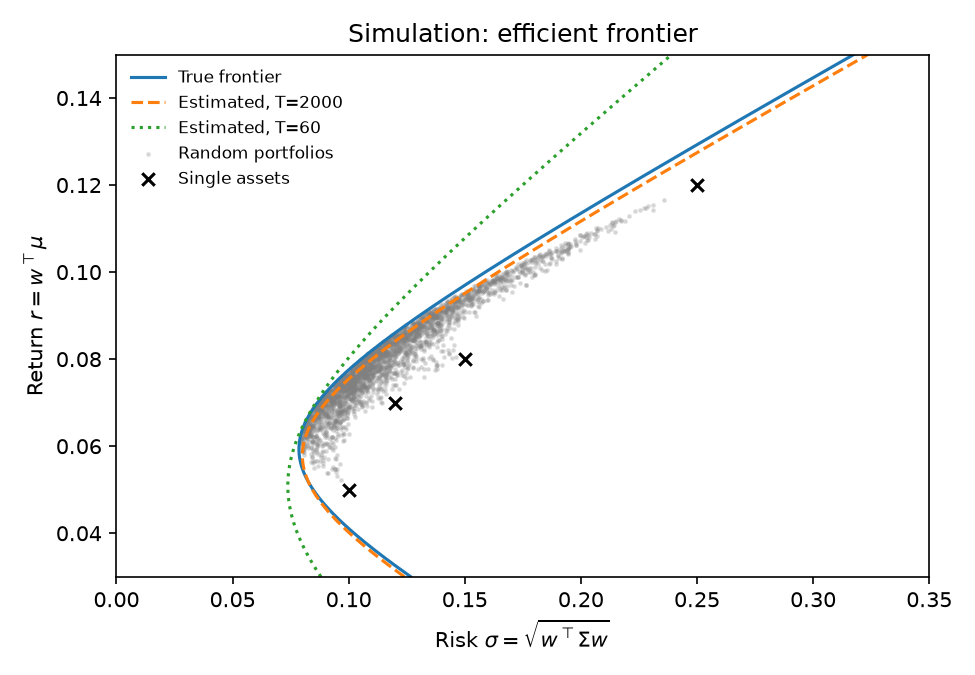
\includegraphics[width=0.7\linewidth]{sim_frontier.png}
\caption{True and estimated efficient frontiers with random portfolios.}\label{fig:frontier}
\end{figure}

\end{document}
